\documentclass[12pt,letterpaper]{hmcpset}
\usepackage[margin=1in]{geometry}
\usepackage{graphicx}
\usepackage{hyperref}

% info for header block in upper right hand corner
\name{Name: \underline{\hspace{4cm}}}
\class{Math 45: Section \underline{\hspace{1cm}}}
\assignment{Assignment 3}
\duedate{4/4/18}

\begin{document}

\begin{problem}
1: (5 points) What linear, second-order, constant-coefficient, unforced DE can have $y(x) =Ce^{-5x} + De^{2x}$ as its general solution? Also, determine the characteristic equation that is
consistent with this general solution.
\end{problem}
\newpage

\begin{problem}
2: (5 points) Complete the following.

\begin{enumerate}
    \item[(a)] Find the solution to the IVP $\ddot{y} + 21\dot{y} + 20y = 0$ with $y(0) = 0$, $\dot{y}(0) = 19$.
    \item[(b)] Your answer to (a) is the sum of two exponential terms. Suppose $t > 0$. As $t$ increases,
which term is negligible and which dominates? Graph your answer to (a) along with
the dominant exponential term by itself on the same axes to verify your answer
\end{enumerate}

\end{problem}
\newpage

\begin{problem}
3: (5 points) Find the general solution to the following ODEs.

\begin{enumerate}
    \item[(a)] $y'' + 6y' + 8y = 0$
    \item[(b)] $y'' + 6y' + 9y = 0$
    \item[(c)] $y'' + 9y = 0$
    \item[(d)] $y'' + 4y = y'$
\end{enumerate}
\end{problem}
\newpage


\begin{problem}
4: (5 points) Consider the IVP $y'' + y' + y = 0$ with $y(0) = 1$ and $y'(0) = 0$.
\begin{enumerate}
    \item[(a)]  Solve this problem using complex exponentials instead of sines and cosines. When you
have solved for your unknown constants, express them in complex exponential form.
(That is, instead of writing it as $a + bi$, write it as $\alpha e^{i\theta}$ for some $\alpha$ and $\theta$.) Leave your
answer in complex exponential form.
    \item[(b)] Now, manipulate your solution in the following way, so as to convert your complex
exponential solution into sines and cosines again. You should get a real-value function
in the end and have a trig function involving a phase shift. Refer to Problem 1 from
Homework 2.

\begin{center}
    $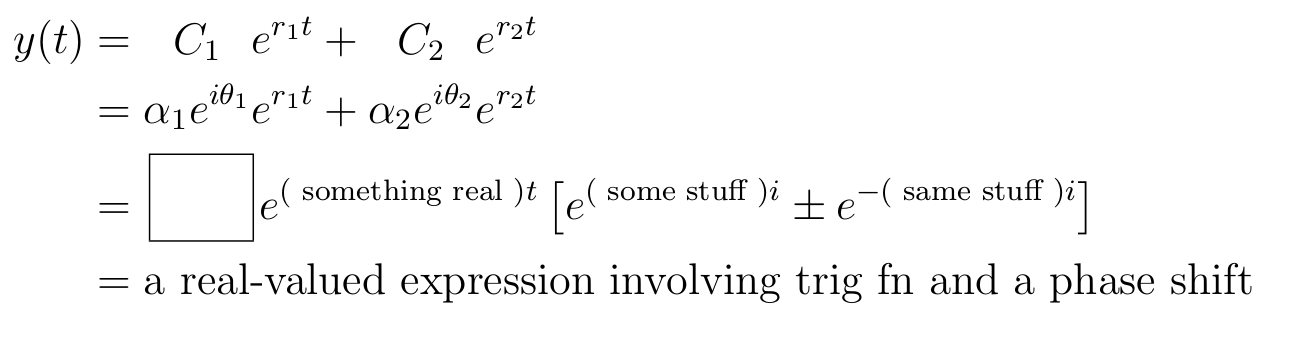
\includegraphics[scale=.3]{HW2work.png}$
\end{center}

    \item[(c)] Compare your solution with the solution that we obtained in class. Show that they are
equivalent.
\end{enumerate}

\end{problem}
\newpage

\begin{problem}
5: (5 points) Consider the second-order, linear, constant-coefficient, unforced DE

\begin{center}
    $ay'' + by' + cy = 0.$
\end{center}

Suppose you know that the solutions to this differential equation decay to $0$ as $t \rightarrow \infty$,
regardless of what initial conditions are chosen. What must be true about the roots of the
characteristic equation $a\lambda^2 + b\lambda + c = 0$? (This question does not require any calculations,
but this idea is important enough that we are highlighting it in this problem.)
\end{problem}
% Add pairs of problems and solutions as needed

\end{document}
